\chapter{Maps of the Chalet room at LPSC}
\label{ch:chalet_appendix}
The ``chalet'' room at LPSC in Grenoble, France, was mapped with the prototype of the mapper (see Ch.\,\ref{ch:mapping}). A panorama of the room is shown in Fig.\,\ref{fig:mapping_lpsc_chalet}. Figure~\ref{fig:mapping_lpsc_chalet_magnitude_map} shows the map of the magnitude of the field. A large dipole source is visible to the right, which was attributed to a large radiator, visible on the photograph below the window on the far wall.

\begin{figure}
  \centering
  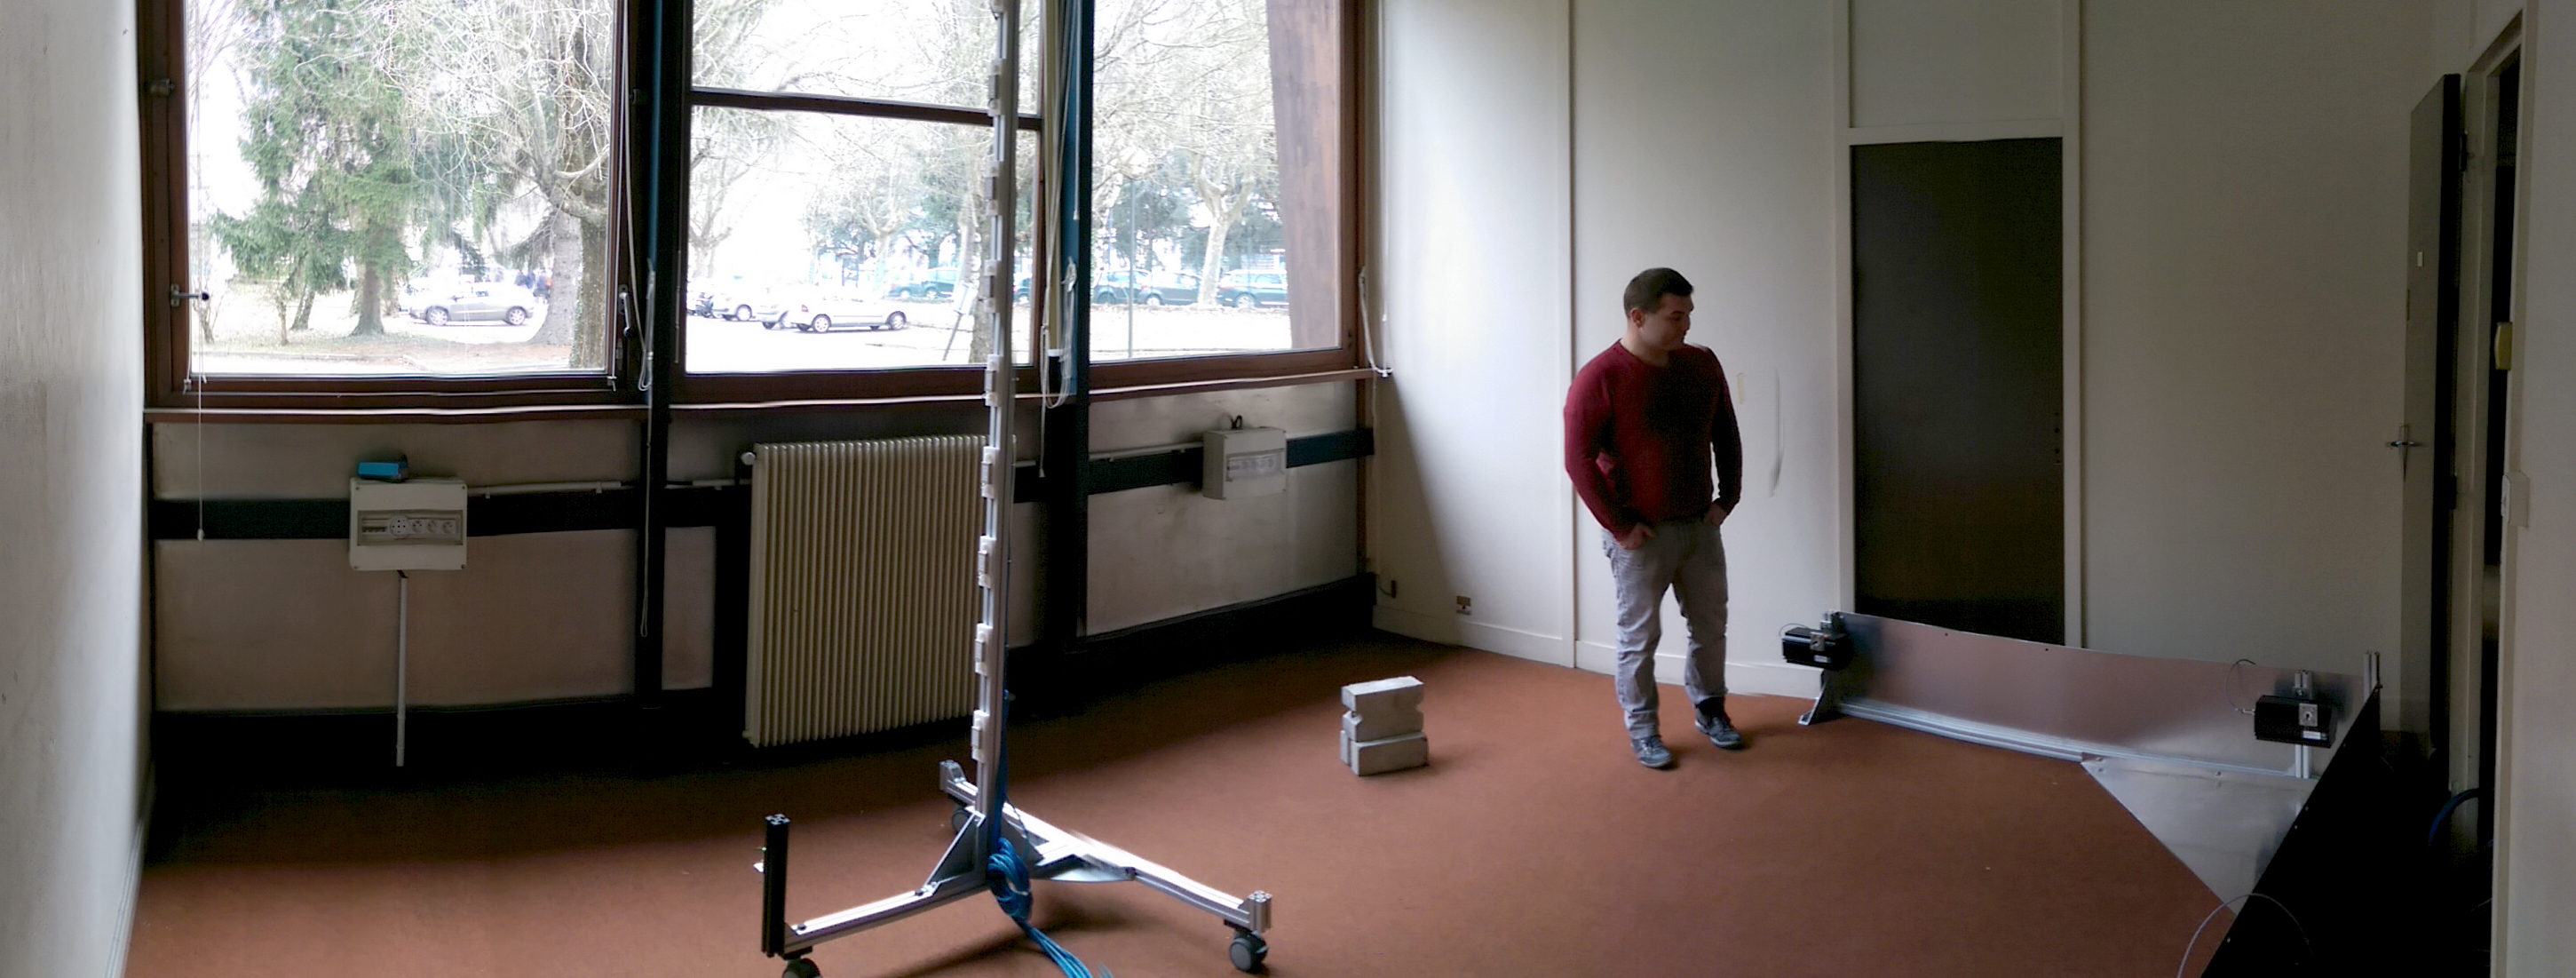
\includegraphics[width=\linewidth]{gfx/mapping/lpsc/chalet_panorama.jpg}
  \caption{A photograph of the ``chalet'' room at LPSC Grenoble. On the picture visible are: the ``L-piece'' holding string potentiometers (to the right), the mapping tower with magnetic field sensors, a large steel radiator (below the window).}\label{fig:mapping_lpsc_chalet}
\end{figure}

\begin{figure}
  \centering
  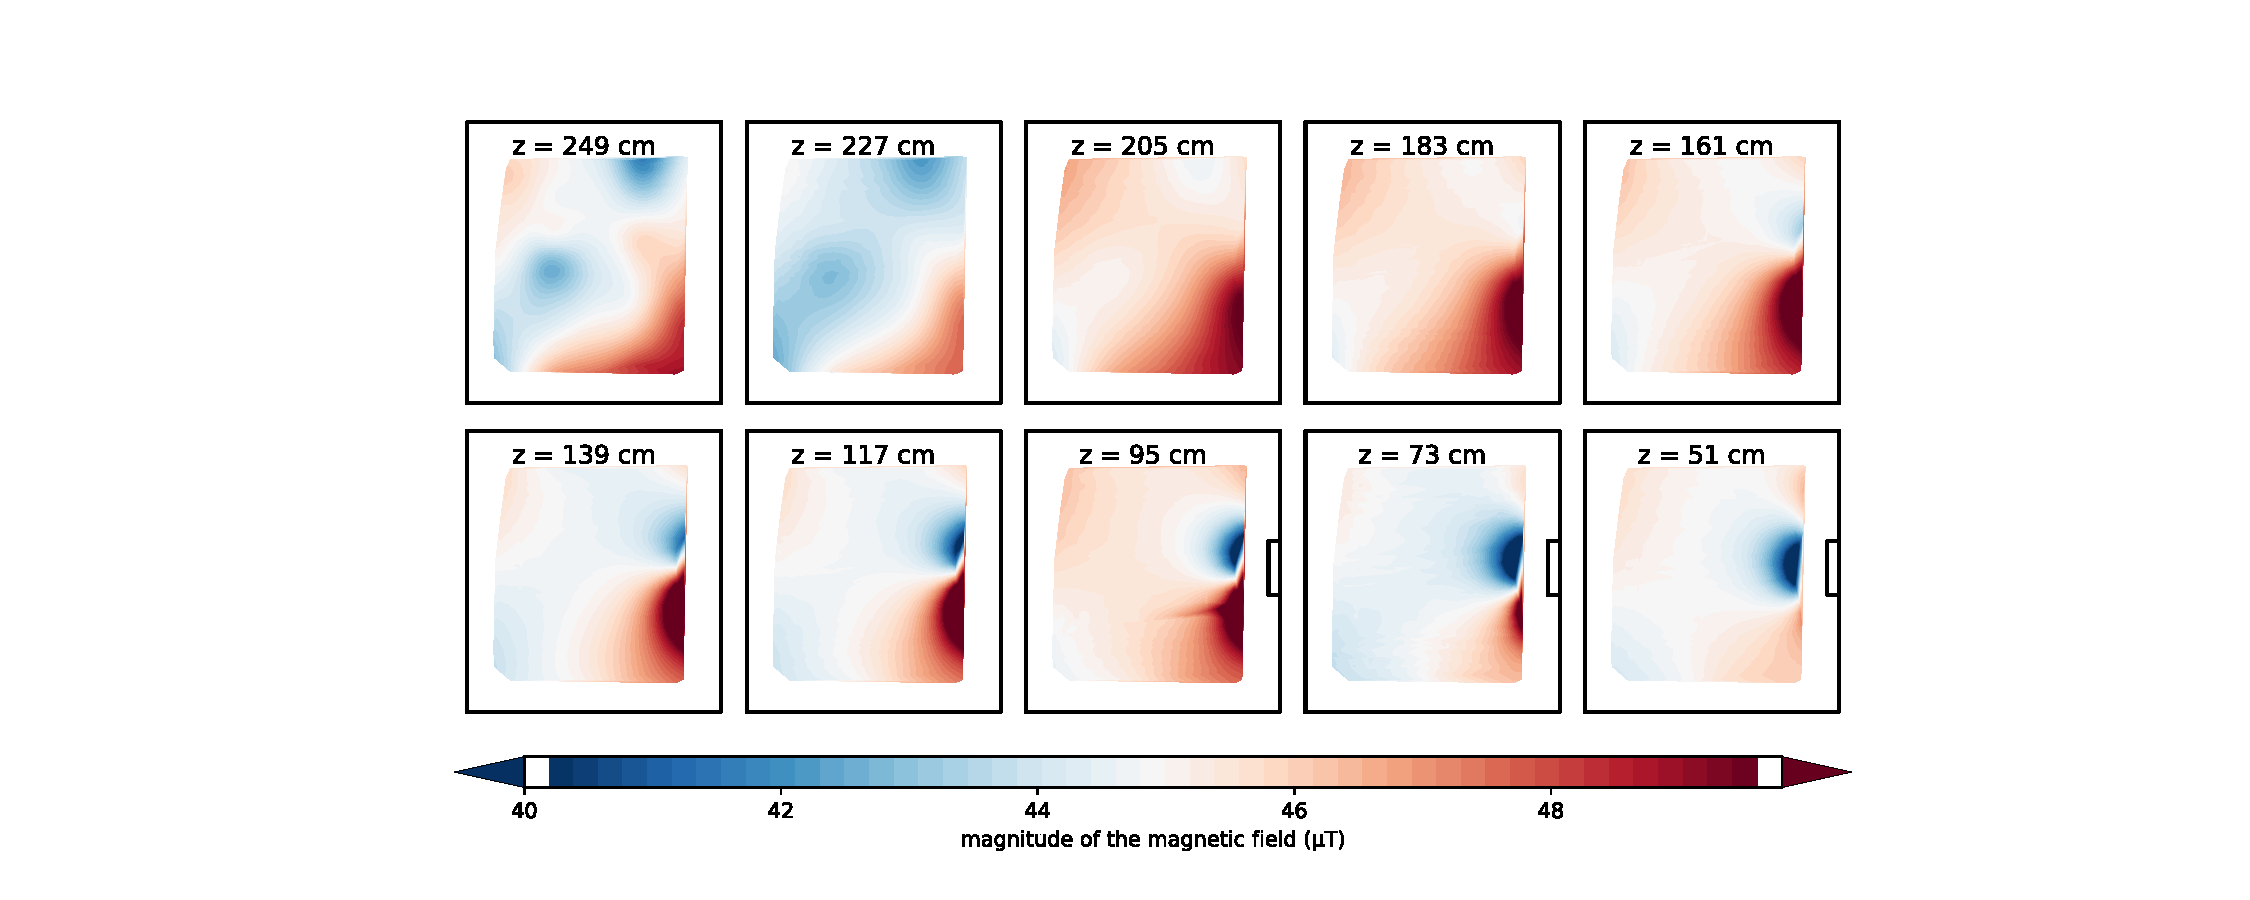
\includegraphics[width=\linewidth]{gfx/mapping/lpsc/chalet.pdf}
  \caption{A map of the magnitude of the magnetic field in the ``chalet'' room at LPSC in Grenoble, France. Each tile depicts measurements in a horizontal plane, as acquired by each sensor.}\label{fig:mapping_lpsc_chalet_magnitude_map}
\end{figure}
